\documentclass{article}
% Change "article" to "report" to get rid of page number on title page
\usepackage{amsmath,amsfonts,amsthm,amssymb}
\usepackage{setspace}
\usepackage{Tabbing}
\usepackage{fancyhdr}
\usepackage{lastpage}
\usepackage{extramarks}
\usepackage{chngpage}
\usepackage{soul,color}
\usepackage{graphicx,float,wrapfig}
\usepackage{multirow}
\usepackage{enumerate}
% In case you need to adjust margins:
\topmargin=-0.45in      %
\evensidemargin=0in     %
\oddsidemargin=0in      %
\textwidth=6.5in        %
\textheight=9.0in       %
\headsep=0.25in         %

% Homework Specific Information
\newcommand{\hmwkTitle}{Tricks for Dirichlet-Multinomial in HDP}
\newcommand{\hmwkClass}{}
\newcommand{\hmwkAuthorName}{Donglai\ Wei}


% Setup the header and footer
\pagestyle{fancy}                                                       %
\lhead{\hmwkAuthorName}                                                 %
\rhead{\firstxmark}                                                     %
\lfoot{\lastxmark}                                                      %
\cfoot{}                                                                %
\rfoot{Page\ \thepage\ of\ \pageref{LastPage}}                          %
\renewcommand\headrulewidth{0.4pt}                                      %
\renewcommand\footrulewidth{0.4pt}                                      %

% This is used to trace down (pin point) problems
% in latexing a document:
%\tracingall

%%%%%%%%%%%%%%%%%%%%%%%%%%%%%%%%%%%%%%%%%%%%%%%%%%%%%%%%\begin{enumerate}

% Some tools
\newcommand{\enterProblemHeader}[1]{\nobreak\extramarks{#1}{#1 continued on next page\ldots}\nobreak%
                                    \nobreak\extramarks{#1 (continued)}{#1 continued on next page\ldots}\nobreak}%
\newcommand{\exitProblemHeader}[1]{\nobreak\extramarks{#1 (continued)}{#1 continued on next page\ldots}\nobreak%
                                   \nobreak\extramarks{#1}{}\nobreak}%

\newlength{\labelLength}
\newcommand{\labelAnswer}[2]
  {\settowidth{\labelLength}{#1}%
   \addtolength{\labelLength}{0.25in}%
   \changetext{}{-\labelLength}{}{}{}%
   \noindent\fbox{\begin{minipage}[c]{\columnwidth}#2\end{minipage}}%
   \marginpar{\fbox{#1}}%

   % We put the blank space above in order to make sure this
   % \marginpar gets correctly placed.
   \changetext{}{+\labelLength}{}{}{}}%

\setcounter{secnumdepth}{0}
\newcommand{\homeworkProblemName}{}%
\newcounter{homeworkProblemCounter}%
\newenvironment{homeworkProblem}[1][Problem \arabic{homeworkProblemCounter}]%
  {\stepcounter{homeworkProblemCounter}%
   \renewcommand{\homeworkProblemName}{#1}%
   \section{\homeworkProblemName}%
   \enterProblemHeader{\homeworkProblemName}}%
  {\exitProblemHeader{\homeworkProblemName}}%

\newcommand{\problemAnswer}[1]
  {\noindent\fbox{\begin{minipage}[c]{\columnwidth}#1\end{minipage}}}%

\newcommand{\problemLAnswer}[1]
  {\labelAnswer{\homeworkProblemName}{#1}}

\newcommand{\homeworkSectionName}{}%
\newlength{\homeworkSectionLabelLength}{}%
\newenvironment{homeworkSection}[1]%
  {% We put this space here to make sure we're not connected to the above.
   % Otherwise the changetext can do funny things to the other margin

   \renewcommand{\homeworkSectionName}{#1}%
   \settowidth{\homeworkSectionLabelLength}{\homeworkSectionName}%
   \addtolength{\homeworkSectionLabelLength}{0.25in}%
   \changetext{}{-\homeworkSectionLabelLength}{}{}{}%
   \subsection{\homeworkSectionName}%
   \enterProblemHeader{\homeworkProblemName\ [\homeworkSectionName]}}%
  {\enterProblemHeader{\homeworkProblemName}%

   % We put the blank space above in order to make sure this margin
   % change doesn't happen too soon (otherwise \sectionAnswer's can
   % get ugly about their \marginpar placement.
   \changetext{}{+\homeworkSectionLabelLength}{}{}{}}%

\newcommand{\sectionAnswer}[1]
  {% We put this space here to make sure we're disconnected from the previous
   % passage

   \noindent\fbox{\begin{minipage}[c]{\columnwidth}#1\end{minipage}}%
   \enterProblemHeader{\homeworkProblemName}\exitProblemHeader{\homeworkProblemName}%
   \marginpar{\fbox{\homeworkSectionName}}%

   % We put the blank space above in order to make sure this
   % \marginpar gets correctly placed.
   }%

%%%%%%%%%%%%%%%%%%%%%%%%%%%%%%%%%%%%%%%%%%%%%%%%%%%%%%%%%%%%%



%%%%%%%%%%%%%%%%%%%%%%%%%%%%%%%%%%%%%%%%%%%%%%%%%%%%%%%%%%%%%
% Make title
\title{\vspace{0.3in}\textmd{\textbf{\hmwkTitle}}}
\date{2010.5.12}
\author{\textbf{\hmwkAuthorName}}
%%%%%%%%%%%%%%%%%%%%%%%%%%%%%%%%%%%%%%%%%%%%%%%%%%%%%%%%%%%%%

\begin{document}
\begin{spacing}{1.1}
\maketitle

\section{0)Problem}
The biggest problem for Dirichlet-Multinomial is that the Energy formula for tables itself does not contain strong clues about the clustering of 
different customers at all. \\ \\
Given the number of customers in every table, the formula does not say anything about the distribution of different customers.\\
Also, the formula favors small number of tables, which can lead wrong direction during the search.\\
(t-term)$ \underline{log \frac{\Gamma(T+\gamma)}{\Gamma(\gamma)}+\sum_{j=1}^{J} \{log \frac{\Gamma(n_{j..}+\alpha)}{\Gamma(\alpha)}-\sum_{t=1}^{m_{j.}}[log(\Gamma(n_{jt.})+log \alpha
]\}}$\\ \\
The hope lies in the "communicating power" among the dishes during {\bf Initialization} and {\bf Searching}.\\
(initialize and search the table config with the auxilary of the config of other {\bf restaurants or dishes})\\ 
\subsection{BAD RESULTS}
Hyperparameters:$\alpha=0.5,\gamma=1.5,\phi_{0}=0.2$\\
Though the probability is close to the ground truth, the config is nothing but junk....
\begin{figure}[h] 
  \begin{minipage}[b]{0.5\textwidth} 
    \centering 
    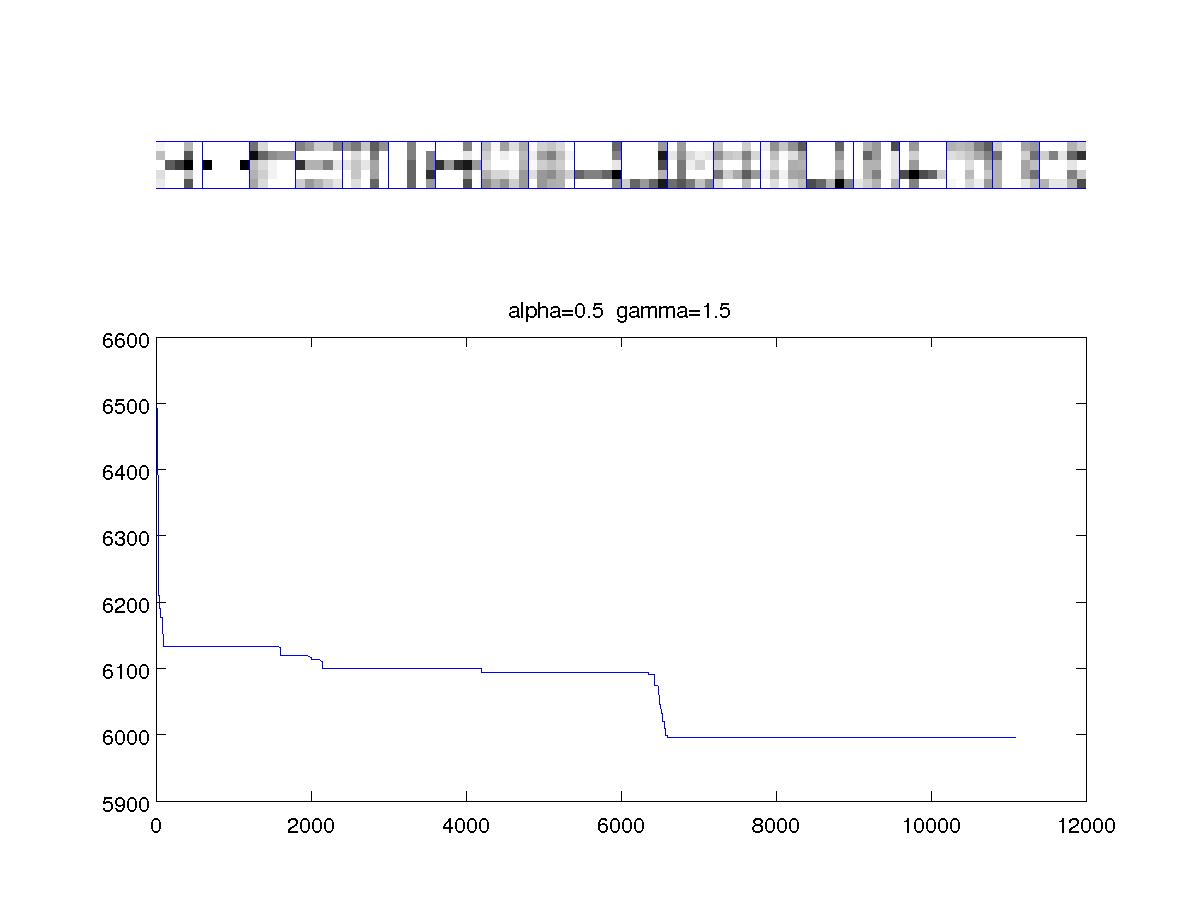
\includegraphics[width=3 in,height=2in]{direct_me.jpg} 
    \caption{ME result: Simply every restaurant has only one table} 
    \label{fig:by:table} 
  \end{minipage}% 
  \begin{minipage}[b]{0.5\textwidth} 
    \centering 
    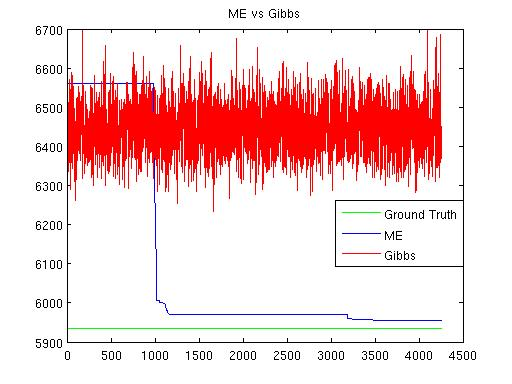
\includegraphics[width=3in,height=2in]{hdp_com2.jpg} 
    \caption{-log probability comparison}
    \label{fig:by:table}  
   \end{minipage}% 
\end{figure}




\section{2) Initialization?}

\subsection{i)Extreme Case}
Bottom-up Initialization: All customers are assigned to different tables with different dishes.\\
Top-down Initialization: Every Restaurant has only one table with the same dish.\\ \\
We know they are of no good since they don't capture potential mixture components.\\ \\
The bad result above uses top-down Initialization.
\subsection{ii)Auxilary Restaurants}
Hoping that some restaurant may have only one mixture component,we have the following initializaiton:\\ \\
For each of the J restaurants independently:\\
\begin{enumerate}
 \item Make J-1 tables serving J-1 dishes, where each dish is informed by all the data from one of the other restaurants
\item  Search over assignments $t_{ji}$ of customers to these tables (keep $k_{jt}$ fixed and don't allow the option of making a new table$\&$dish not shared with any other restaurant)
\item  Store the at most J-1 tables with at least one customer (hopefully this will be a number bigger than one but much less than J-1)
\end{enumerate}
But the problem is we are still assigning the customer too greedily, which does not capture the distribution of different words:\\ 
Actually, {\bf it is equivalent to simply assigning customers with the same type(word) to the same table.} \\
The difference among the k-term happens at $log\frac{1}{\Gamma(\phi_{0}+n_{..k}^{w_{0}})}$ which is concave(bigger $n_{..k}^{w_{0}}$,bigger decrease)\\
Thus assign the first customer to the auxilary restaurant with the highest count of word $w_{0}$ will mostly decrease the Free Energy(Negative log Probability).
\begin{figure}[h] 
  \begin{minipage}[b]{0.5\textwidth} 
    \centering 
    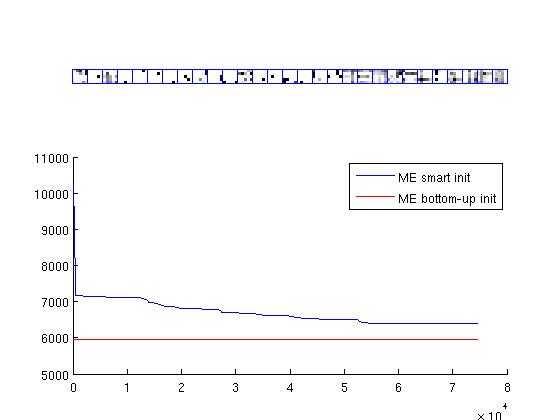
\includegraphics[width=3in,height=2in]{greed.jpg} 
    \caption{Auxilary Restaurants Initialization ends up with smaller dishes} 
    \label{fig:by:table} 
  \end{minipage}% 
  \begin{minipage}[b]{0.5\textwidth} 
    \centering 
    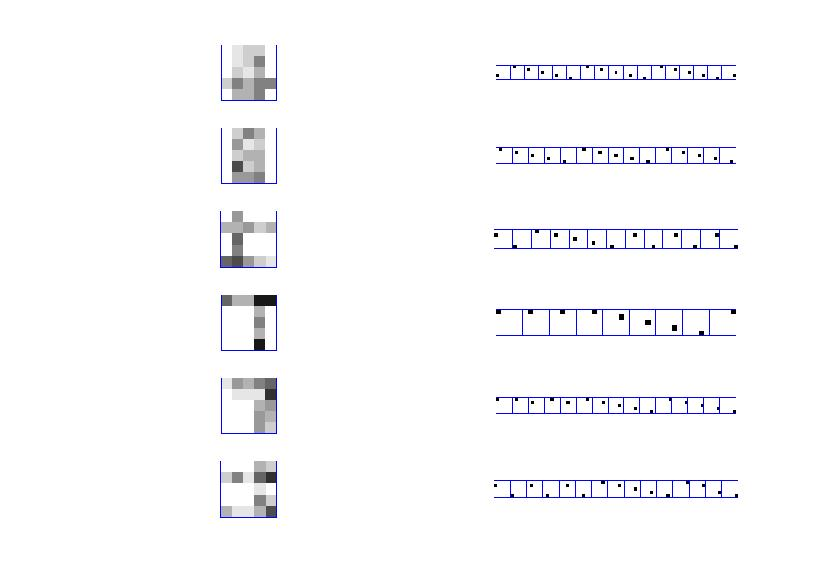
\includegraphics[width=3in,height=2in]{greed_init.jpg} 
    \caption{Initialization for the first six restaurants(left)with table config(right)}
    \label{fig:by:table}  
   \end{minipage}% 
\end{figure}


\subsection{iii)Gibbs Initialization}
One step back, let's see if initializaiton really matters.\\
Start with an "almost done" Gibbs sampling(500 runs) result, below is the comparison of table configs for the first five restaurants.\\
\begin{figure}[h] 
  \begin{minipage}[b]{0.5\textwidth} 
    \centering 
    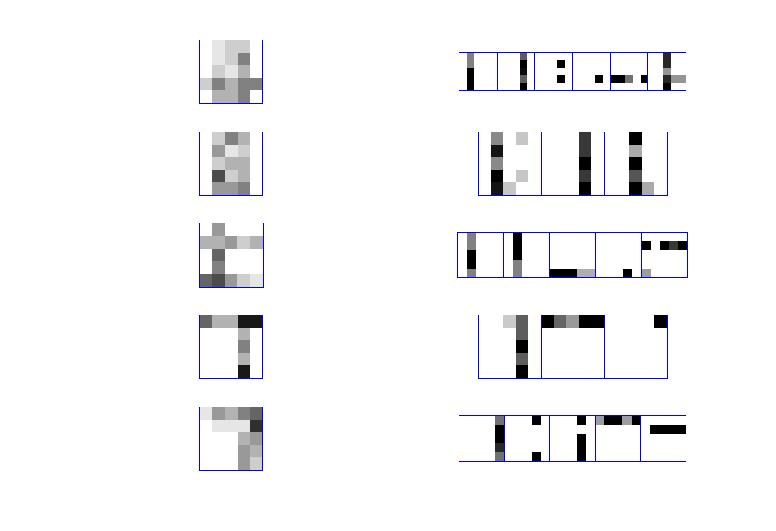
\includegraphics[width=3in,height=2in]{gibb_part.jpg} 
    \caption{Crude Gibbs Sampling results} 
    \label{fig:by:table} 
  \end{minipage}% 
  \begin{minipage}[b]{0.5\textwidth} 
    \centering 
    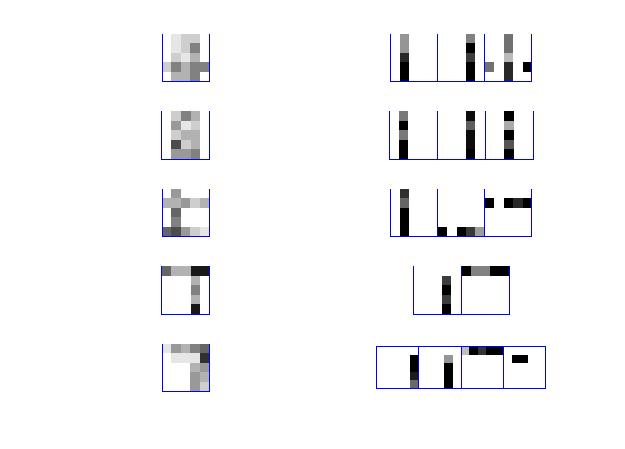
\includegraphics[width=3in,height=2in]{gibb_me_part.jpg} 
    \caption{ME results with Gibbs Initialization}
    \label{fig:by:table}  
   \end{minipage}% 
\end{figure}
\begin{center}
    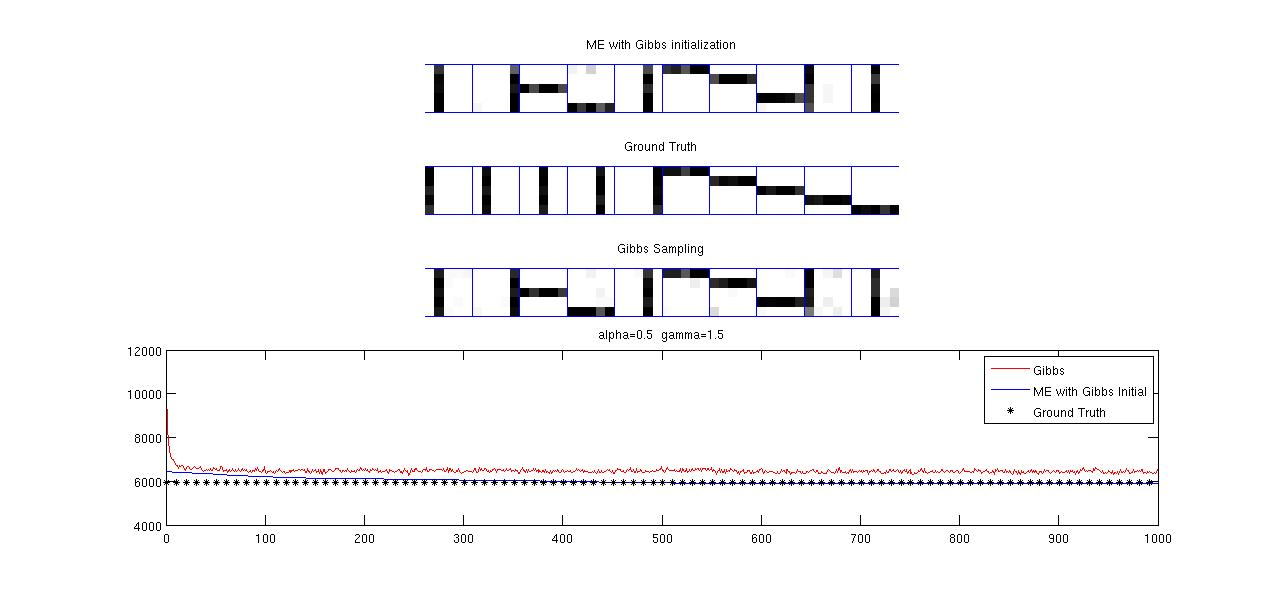
\includegraphics[width=6in,height=3in]{gibbs_end.jpg} 
\end{center}
\begin{enumerate}
\item With rough idea of how the dishes look like, ME algorithm works.
\item Noticably, ME algorithm can group small tables correctly and efficiently by minimizing Free Energy, while it may take longer time for Gibbs sampling.
\end{enumerate}



\subsection{iv)Finer Auxilary Restaurants}
Intuition:(improve the rough Auxilary Restaurants)\\
\begin{enumerate}
\item (Inspired by Gibbs Initialization) We only need to divide each restaurant into {\bf small reliable} tables and ME can do the rest.\\
\item (Inspired by Auxilary Restaurants)Assigning cutomers one by one may be too greedy, we may try to group them first according to auxilary restaurants.\\
(In other words, it may be too utopia that some restaurant is made of one bar, but it could probably happen that the intersection of 2 restaurants may be part of the bar)
\end{enumerate}
So, the idea is: e.g. Given other 39 mixtures of bars, split a mixture of bars into reasonable parts(unoverlapped) and assign customers to them.\\ \\

Psuedocode:How to find the parts of a Restaurant(R)\\ \\
Preposessing: find the overlapped regions with other Restaurants.\\
While there are still words in R unassigned to parts
\begin{enumerate}
\item 
\begin{enumerate}[(a)]
\item Top-down: define the part as the biggest overlapped region
\item (or)Bottom-up: define the part as the smallest overlapped region containing (R-biggest overlapped region)
\end{enumerate}
\item assign words falling into the new part to it.
\item R=R-part;Overlapped Region=Overlapped Region-part
\end{enumerate}
end\\ \\

(I choose the bottom-up approach)Below, we can see that the heuristic initializaiton works to some degree(Fig 7), but the result is still not good.\\
From Fig 8, we can see that the problem lies in {\bf splitting tables}.\\
From Fig 9, we can see that the correct dishes are found and we only need to {\bf split and merge the noise}.\\
Since we can not expect too much from the initializaiton, we have to improve our searching methods.

\begin{figure}[h] 
  \begin{minipage}[b]{0.5\textwidth} 
    \centering 
    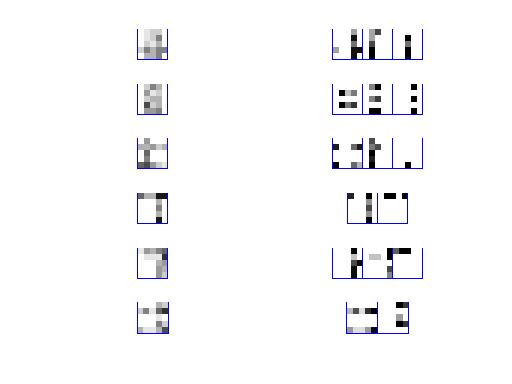
\includegraphics[width=3in,height=2in]{shape_init.jpg} 
    \caption{Finer Auxilary Restaurants(FAR) Initialization} 
    \label{fig:by:table} 
  \end{minipage}% 
  \begin{minipage}[b]{0.5\textwidth} 
    \centering 
    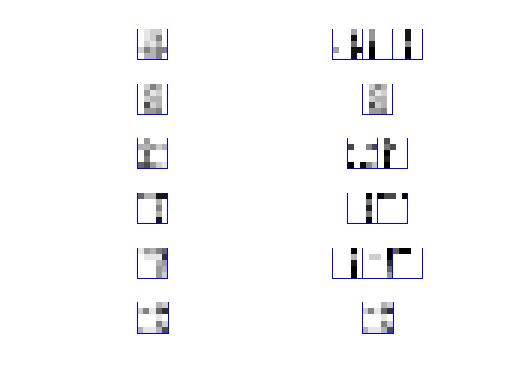
\includegraphics[width=3in,height=2in]{shape_end.jpg} 
    \caption{ME results with (FAR) Initialization}
    \label{fig:by:table}  
   \end{minipage}% 
\end{figure}
\begin{figure}[h] 
    \centering 
    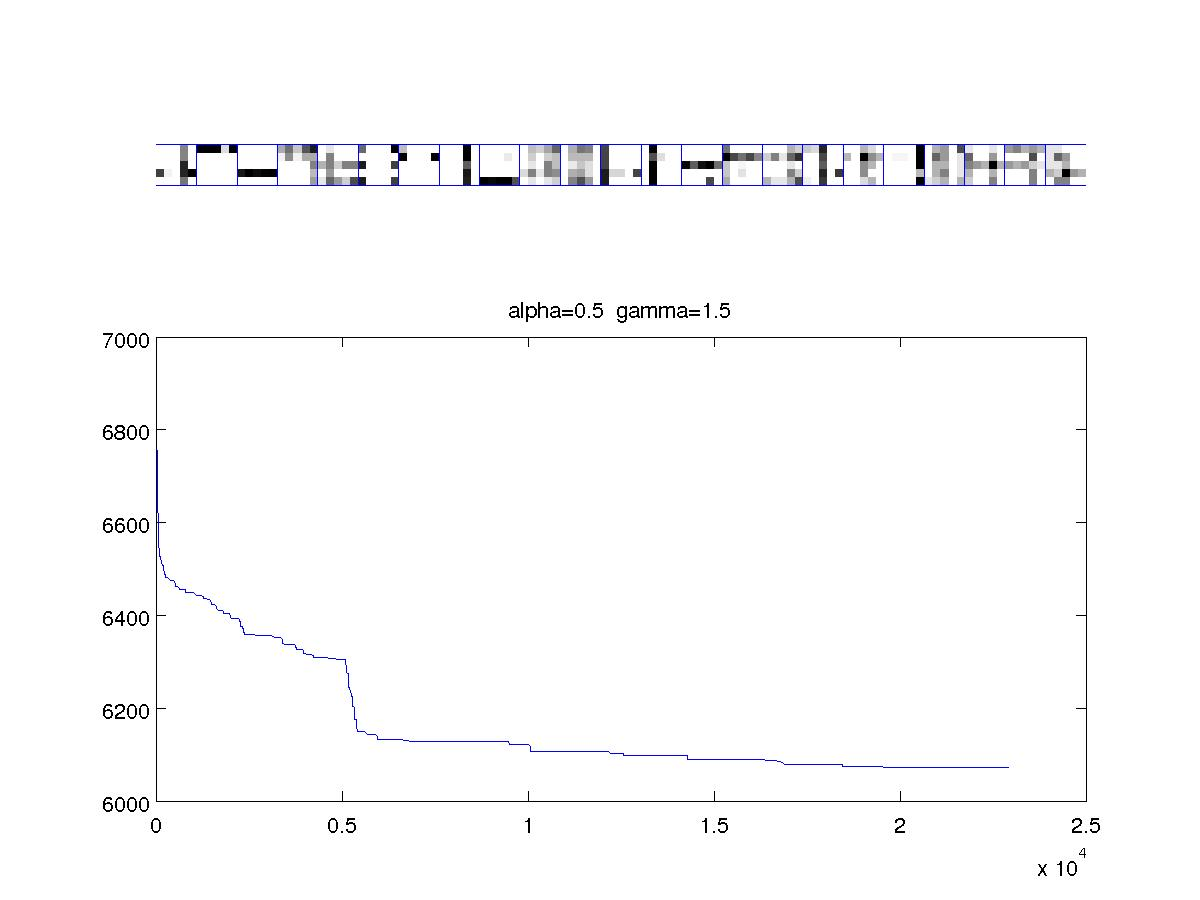
\includegraphics[width=5in,height=3in]{shape.jpg} 
    \caption{ME results with (FAR) Initialization}
    \label{fig:by:table} 
\end{figure}





\section{}
\section{}
\section{}







\section{3) Searching Scheme?}

\subsection{0) A Little Modification of Spliting dishes}
In order to encourage splitting the noisy dishes, we allow merging new dishes to other dishes during the split.
\subsection{i) Spliting tables with Auxilary Dishes}
From Fig8, we can see that previous algorithm to split tables doesn't do a good job.\\
Preivously:
\begin{enumerate}
\item Use 2-means++ to split a table into 2 new tables with new dishes 
\item Iteratively local search the table for customers and local search dishes for the 2 new tables
\end{enumerate}
For Normal-Inverse-Wishart-Gaussian case, two-means++ works well because the new tables will penalize for the "inconsistency" of the data themselves.\\
For Dirichlet-Multinomial case, however, we know that the tables only care about the number of customers instead of their types(words).\\
So the first step in the alogrithm breaks down by producing super big and super small tables...\\ \\
Inspired by Initialization with auxilary restaurants, we can {\bf split tables with auxilary dishes}!!!(same pseudo-code)\\

Below, we can see that split with auxilary dishes does a little better to split the tables.\\
But still, we have noisy dishes in Fig12.

\begin{figure}[h] 
  \begin{minipage}[b]{0.5\textwidth} 
    \centering 
    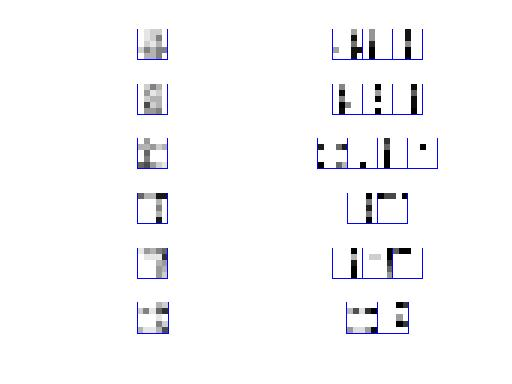
\includegraphics[width=3in,height=2in]{shape_local_end.jpg} 
    \caption{split with auxilary dishes with (FAR) Initialization}
    \label{fig:by:table} 
  \end{minipage}% 
  \begin{minipage}[b]{0.5\textwidth} 
    \centering 
    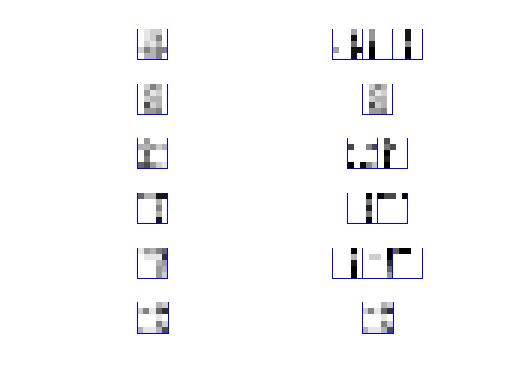
\includegraphics[width=3in,height=2in]{shape_end.jpg} 
    \caption{normal split with (FAR) Initialization}
    \label{fig:by:table}  
   \end{minipage}% 
\end{figure}
\begin{figure}[h] 
    \centering 
    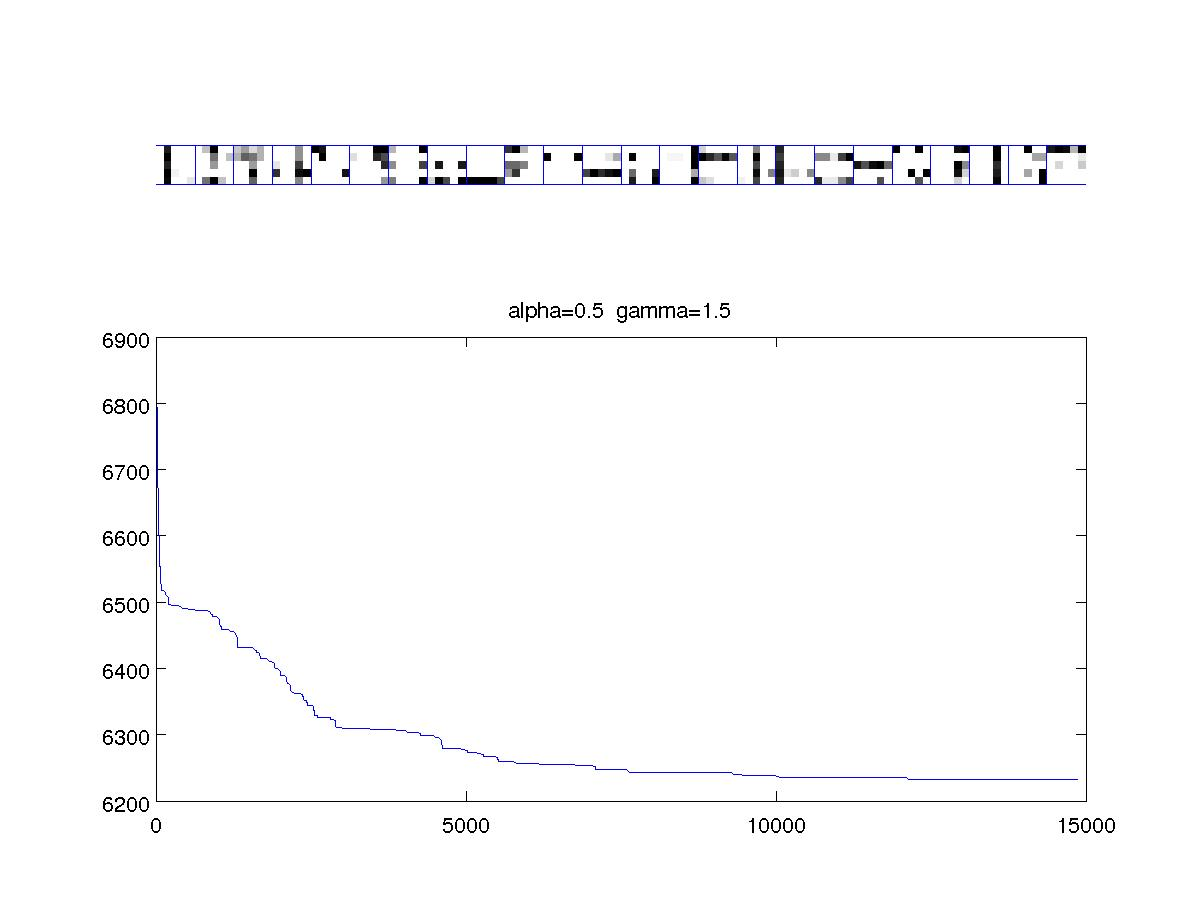
\includegraphics[width=5in,height=3in]{shape_local_split.jpg} 
    \caption{ME results with (FAR) Initialization}
    \label{fig:by:table} 
\end{figure}

\subsection{ii) Spliting tables with damped "t-term"}
In Fig10, it seems natural to split the first table in the third restaurant according to the "right dishes".\\
But the problem is assigning the splitted tables to correct dishes does not decrease enough Free energy.\\
For most of the time, splitting tables increase a little more free energy.(Creating the potential well)\\ \\
Since we may benifit from smaller tables, we can split tables with damped "t-terms".\\
Instead of judging the split move by "$\Delta$t-term+$\Delta$k-term$<$0", we can use "$\alpha \Delta$t-term+$\Delta$k-term$<$0"\\
where $\alpha \in (0,1)$\\ \\ \\
Well,IT WORKS!!!!! Below are two different runs with $\alpha=0.7$:
\begin{figure}[h] 
  \begin{minipage}[b]{0.5\textwidth} 
    \centering 
    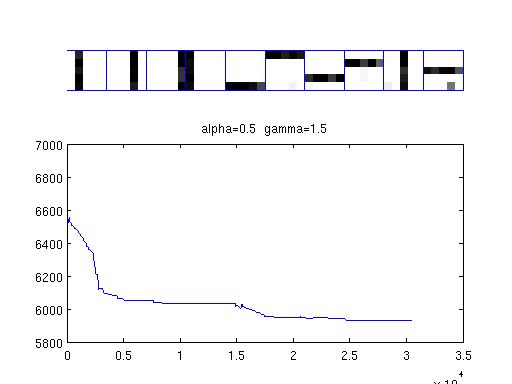
\includegraphics[width=3in,height=2in]{shape_damped_split.jpg} 
    \caption{damp+auxilary dishes+(FAR) Initialization}
    \label{fig:by:table} 
  \end{minipage}% 
  \begin{minipage}[b]{0.5\textwidth} 
    \centering 
    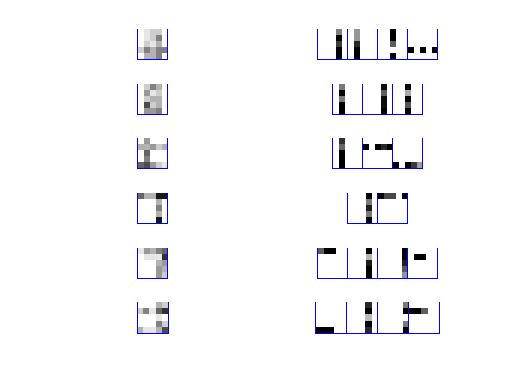
\includegraphics[width=3in,height=2in]{shape_damp_end.jpg} 
    \caption{normal split with (FAR) Initialization}
    \label{fig:by:table}  
   \end{minipage}% 
\end{figure}
\begin{figure}[h] 
  \begin{minipage}[b]{0.5\textwidth} 
    \centering 
    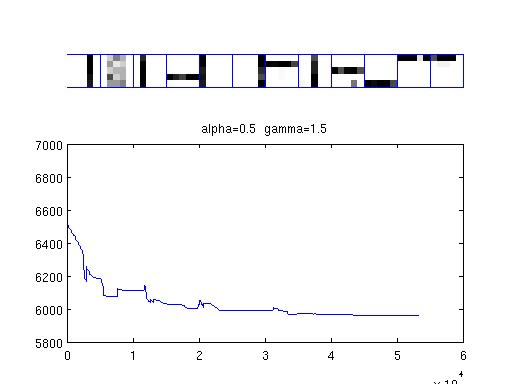
\includegraphics[width=3in,height=2in]{shape_damped_split_2.jpg} 
    \caption{damp+auxilary dishes+(FAR) Initialization}
    \label{fig:by:table} 
  \end{minipage}% 
  \begin{minipage}[b]{0.5\textwidth} 
    \centering 
    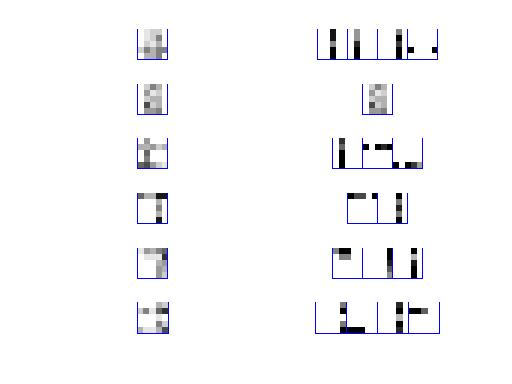
\includegraphics[width=3in,height=2in]{shape_damp_end_2.jpg} 
    \caption{normal split with (FAR) Initialization}
    \label{fig:by:table}  
   \end{minipage}% 
\end{figure}

\subsection{iv) Extras}
Previously, I was a little inconfident about the "damped t-term" and only ran it with fewer iterations, which "as expected" doesn't provide good result.\\ \\
So I came up with two extra methods...\\ \\

\begin{enumerate}
\item {\bf "Spliting tables with Re-initializaiton"}\\
The problem is that we have found the true dishes(10) and the problem is to get rid of the noisy ones(~10).\\
Simply, instead of struggling with splitting tables and dishes, we can start it over again!!\\ \\
Remember,we achieve this only by initializing with naive parts. So we can reinitialize with current dishes!!!\\ \\
As expected, true dishes have bigger chance to be selected~~
\begin{figure}[h] 
  \begin{minipage}[b]{0.3\textwidth} 
    \centering 
    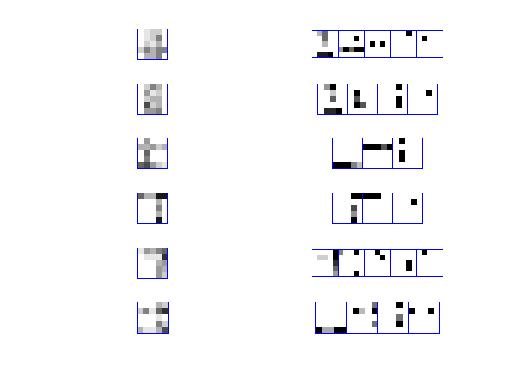
\includegraphics[width=2in,height=2in]{2_init_part.jpg} 
    \caption{first six restaurants after Reinitialization}
    \label{fig:by:table} 
  \end{minipage}% 
  \begin{minipage}[b]{0.3\textwidth} 
    \centering 
    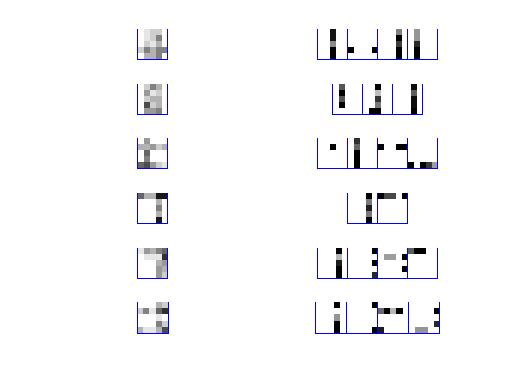
\includegraphics[width=2in,height=2in]{2_init_part_end.jpg} 
    \caption{first six restaurants after iterations}
    \label{fig:by:table}  
   \end{minipage}% 
\begin{minipage}[b]{0.3\textwidth} 
    \centering 
    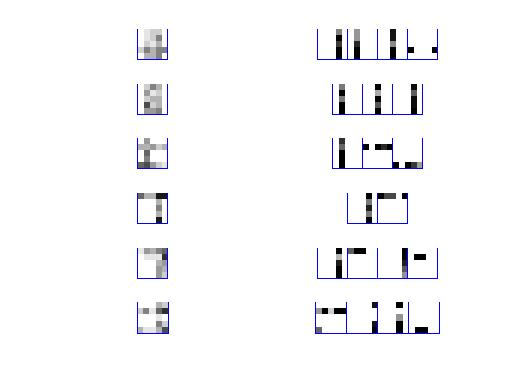
\includegraphics[width=2in,height=2in]{2_init_part_end2.jpg} 
    \caption{first six restaurants after iterations(another run)}
    \label{fig:by:table}  
   \end{minipage}% 
\end{figure}
\begin{figure}[h] 
  \begin{minipage}[b]{0.5\textwidth} 
    \centering 
    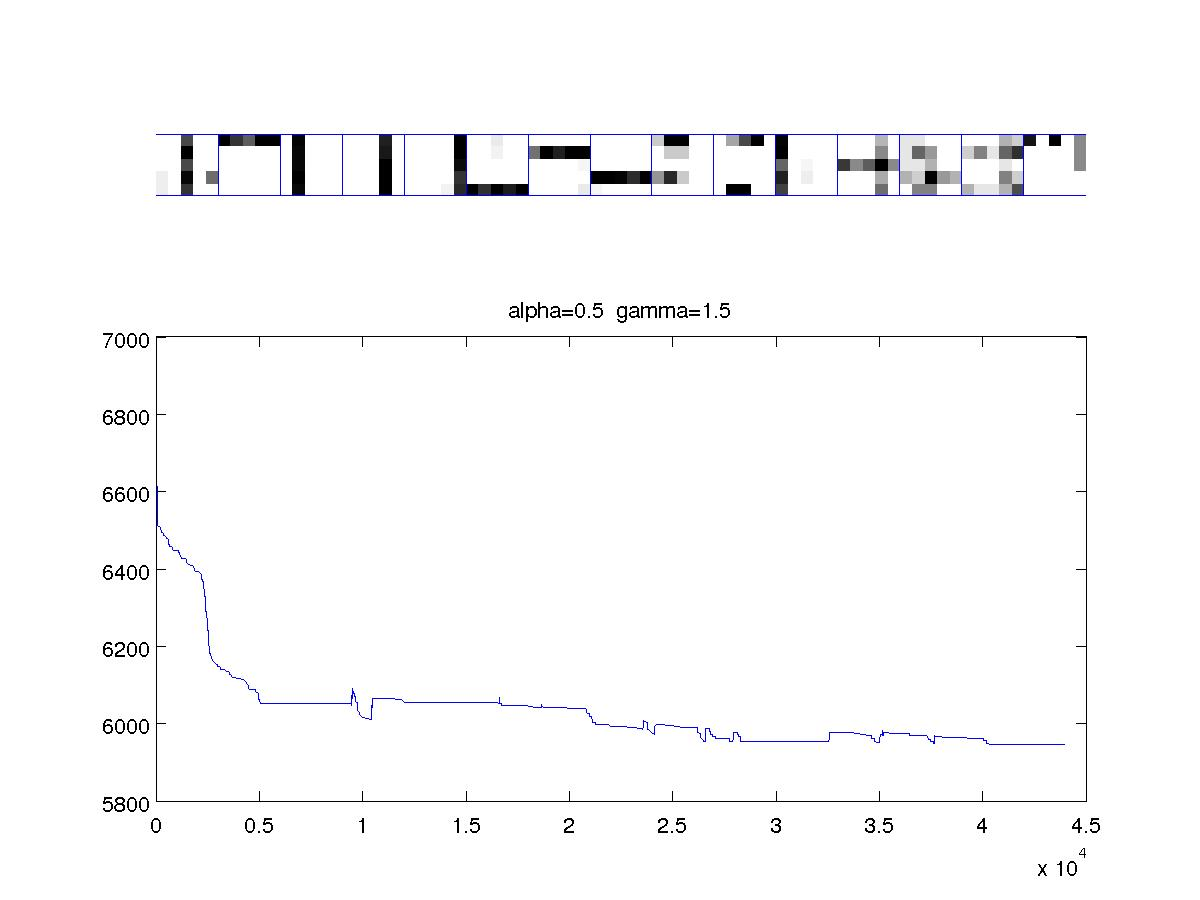
\includegraphics[width=3in,height=2in]{2_init_p.jpg} 
    \caption{damp+auxilary dishes+(FAR) Initialization}
    \label{fig:by:table} 
  \end{minipage}% 
  \begin{minipage}[b]{0.5\textwidth} 
    \centering 
    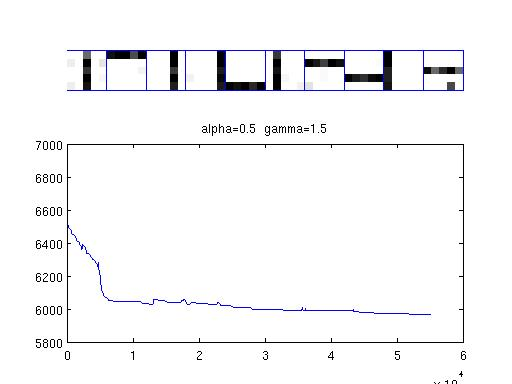
\includegraphics[width=3in,height=2in]{2_init_p2.jpg} 
    \caption{normal split with (FAR) Initialization}
    \label{fig:by:table}  
   \end{minipage}% 
\end{figure}





\item {\bf "The Grand Split"}
As we mentioned before, we can do a "grand" split of tables instead of do it locally.\\
Previously, we judge the split table move one restaurant after another independently, now we split them all and find better config for them.\\ \\
But it doesn't work significantly well...

\end{enumerate}






\end{spacing}
\end{document}

%%%%%%%%%%%%%%%%%%%%%%%%%%%%%%%%%%%%%%%%%%%%%%%%%%%%%%%%%%%%%
